\chapter{DATA C100: Cross Validation}

\section{Variance and Training Error}
When attempting to form a model for predicting new datapoints, say linear regression, we often have some way to find optimal parameters. \\
The process of finding these parameters that lead to the best predictions possible is known as \textbf{training}, and the dataset used for this process is known as the \textbf{training set}.\\
However, even the model itself would then have some errors when compared to the original data. This error is known as the \textbf{training error}. \\
To reduce training error, we might sometimes make the model more complex, so it covers more ground by using more information from a data entry and can end up making better predictions. The sensitivity of our model towards its fata is known as \textbf{variance}. \\
Of course, we can try to make a model entirely correct when applied onto the data we train it on. For an $n$-point dataset, we can use a $n-1$ degree polynomial that passes through all $n$ points of the dataset. At that point, the model has high variance, high complexity, and virtually $0$ training error. \\
But then, is this model use-able on other real-world data whose behavior deviates from the dataset?

Machine Learning scientists have developed the following famous diagram to discuss such phenomenon:
\begin{ln-fig}{Variance-Training Error Tradeoff}{}
    \begin{center}
        \includegraphics[scale=0.4]{figs/ln06/var-train-err-tradeoff.png}
    \end{center}
\end{ln-fig}

When a model \textbf{overfits}, it refers to the phenomenon discussed above: the model is aggressively tailored towards the dataset and fails to predict data outside the dataset it's trained on. \\
Allow me to quote an insight from some other articles I've written, on a puppy vs. bagel classifier model, to address why is not testing the model after training a bad idea:
\begin{quote}
    This is because if a model uses too much data from training set, then its formula will be extremely tailored to the reality that training set captures.
    However, we have no way to decide if training set provides a good image on how reality looks like.
    
    For example, if my training set only has pictures of blue puppies and blue bagels, my test set is responsible of telling me there exist many puppies and bagels that are not blue.
    
    If a model only follows its training set and behaves excessively inaccurate on the testing set and real-world data, we call the model as “overfitting” the training set.
    In other words, the model overly fits the training set and lives in the world shaped by that training set, unaware of what the truth is regarding the distinction of puppies and bagels.
    
    Therefore, a partition of the original dataset still needs to be used for testing, and another portion used for training. A popular choice of train-test split is 7:3.
\end{quote}
In this case, even if we do attain a zero MSE, the model is useless outside the dataset we have trained on.

\section{Validation}
Scientists then came up with an idea: what if we attempt to validate our model using extra data point? \\
The first brief method that came into mind is a ``holdout method'', where for a datset of 100 points, we use 70 of 100 on training the data, which we call the \textbf{training set} (as in the dataset on which we train the model), and hold 30 of it out. \\
Once again, this 7:3 ratio is just a common convention. The default holdout ratio for sklearn is 3:1, and some other practitions using 4:1 also exist. \\

So after training the dataset on the 70 data points, we test our model on the rest 30 which we have not trained on. This set of held out data is often called the \textbf{validation set} (or alternatively, development set, ``dev set''). \\
This allows us to validate our model by seeing how it behaves when predicting data outside the dataset we trained the model on. For the technology in DATA C100, its computation is as follows:
\setbox\codebox=\hbox{
    \begin{lstlisting}
    >>> from sklearn.utils import shuffle
    >>> training_set, dev_set = np.split(shuffle(df), [70])
    \end{lstlisting}
}
\begin{ln-code}{Hold-Out Dataset in Python}{}
    \usebox\codebox
\end{ln-code}
Ideally, we then arrive at what the following diagram describes:
\begin{ln-fig}{Variance-Erroe Tradeoff}{}
    \begin{center}
        \includegraphics[scale=0.4]{figs/ln06/var-err-tradeoff.png}
    \end{center}
\end{ln-fig}
where we attempt to use a model whose complexity allows the minimum training error and validation error.

In this case, the degree of predictor variables, which form a polynomial for the regression line, is what we can blame and adjust for the deficiency of our model in overfitting. 

In machine learning, these variables that influence the learning process as outlined by the above tradeoff diagram is called \textbf{hyperparameter}. This can also involve, for example, the ratio of number of data in training set to that in validation set.

There is also an inherent problem with this hold-out idea, which we will address in the following section.

\section{K-Fold Cross Validation}
If we continue to use the same validation set for every single time we test our data, then our data would also be tailored towards the validation set. This causes a similar mistake to overfitting. \\
To address this issue, let us consider another similar approach of valiation, called \textbf{K-Fold Cross Validation}.

Imagine that we have divided our entire dataset into $k$ equal partition:
\begin{ln-fig}{K-Fold Cross Validation Sets}{}
    \begin{center}
        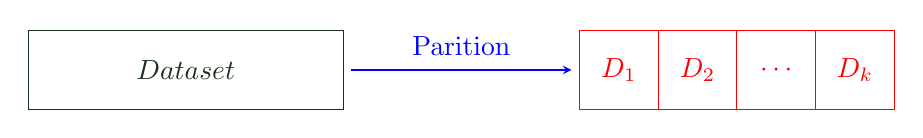
\begin{tikzpicture}
            \draw[green!10!black!90!]
                (0, 0) rectangle (4, 1)
                (2, 0.5) node{$Dataset$};
            \draw[blue]
                [-stealth](4.1, 0.5) -- (6.9, 0.5);
            \draw[blue]
                (5.5, 0.8) node{Parition};
            \draw[red]
                (7, 0) rectangle (8, 1)
                (7.5, 0.5) node{$D_1$}
                (8, 0) rectangle (9, 1)
                (8.5, 0.5) node{$D_2$}
                (9, 0) rectangle (10, 1)
                (9.5, 0.5) node{$\cdots$}
                (10, 0) rectangle (11, 1)
                (10.5, 0.5) node{$D_k$};
        \end{tikzpicture}
    \end{center}
\end{ln-fig}
Then, for each $i \in \{1, \cdots, k\}$, let us use the partition of dataset $D_i$ as our validation set to train the model. Denote the resulting validation error as ${VE}_i$. \\
Record such value from ${VE}_1$ to ${VE}_k$, and note the average of these validation errors as the overall validation error of training this model. \\
This way, we managed to validate our model without being stuck with one same validation set, and can provide a much more objective review towards the quality of current model complexity.

Popular choices of such value $k$ would be $5$, $10$, and $N$ (the length of the entire dataset). \\
In the case we have chosen to perform $N$-fold cross validation, which is also known as ``leave one out cross validation'', each point becomes a validation set and will usually yield the greatest result.
However, it is computationally expensive. \\
On the other hand, using $k = 5$ offers a less ideal result in tradeoff with a smaller computational cost.
\setbox\codebox=\hbox{
    \begin{lstlisting}
    GridSearchCV
    Args:
        estimator: The model for finding optimal parameters.
        param_grid: Hyperparameters stored in a dictionary.
        scoring: The loss function by which we assess performance
        of hyperparameters, usually "neg_mean_squared_error"
        cv: number of folds, or a 2D list containing indices
        for training set and dev set.
    Returns:
        The optimal parameters for estimator specified.
    \end{lstlisting}
}
\begin{ln-code}{Hold-Out Dataset in Python}{}
    \usebox\codebox
\end{ln-code}

\section{Test Set}
While we may find the model with the best validation set loss as the optimal one we will use in real life, when reporting the model on a public occassion (say paper, or actual incorporation with some procedure), we would like to assess our model using a special test set that we have never seen or used for any purpose. \\
This also relates back to how we preferred cross validation over hold-out on most occassions: avoiding biases towards the validation set used. \\
A test set can be easily produced via partitioning our original dataset into the \textbf{Training Set}, \textbf{Validation Set}, and \textbf{Testing Set}. We usually have some habits in how to partition a dataset into these subsets, such as producing a 70-15-15 partition.

To incorporate testing set into the big-picture of learning process with error-variance tradeoff, let's referrence this visual from DATA C100:
\begin{ln-fig}{Variance-Training Error Tradeoff}{}
    \begin{center}
        \includegraphics[scale=0.4]{figs/ln06/var-test-err-tradeoff.png}
    \end{center}
\end{ln-fig}
We may see that the only difference between testing error and validation error is essentially how restrictive the computation of those error is, as we are, for testing purposes, neither allowed nor supposed to access the error curve for testing set.
